\documentclass[10pt]{beamer}
\usetheme[progressbar=foot]{metropolis}
\usepackage{amsmath}
\usepackage{minted}
\usepackage{tikz}\usetikzlibrary{shapes,arrows,calc}

\title{Static analysis for API error detection in IoT devices}
\subtitle{Tapioca: a library for reasoning about web requests at compile-time}
\date{28 June 2017}
\author{Oliver Ford}
\institute{Imperial College London}

\makeatletter
\setlength{\metropolis@progressinheadfoot@linewidth}{1pt}
\makeatother

\begin{document}
\setbeamertemplate{frame footer}{\insertsection}

{
\setbeamerfont{title}{size=\large}
\setbeamerfont{subtitle}{size=\small}
\maketitle
}

\begin{frame}{Contents}
  \setbeamertemplate{section in toc}[sections]
  \tableofcontents[hideallsubsections]
\end{frame}

\section{Motivation}

\begin{frame}{Errors in device communication}

    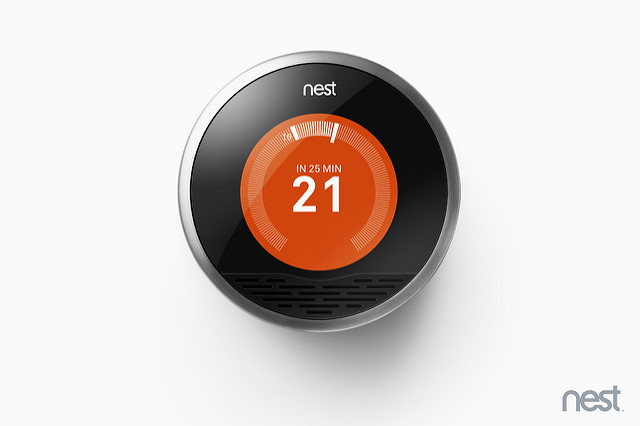
\includegraphics[width=\textwidth]{images/nest}

\end{frame}

\begin{frame}{Who will notice?}

    \begin{itemize}[<+->]
        \item Many IoT devices have no user-facing display
        \begin{itemize}
            \item and may not report an error anyway
        \end{itemize}
        \item Server operator might notice
        \begin{itemize}
            \item but that may not be the device manufacturer
        \end{itemize}
    \end{itemize}
    \onslide<+->{\begin{examples}
        \begin{itemize}[<+->]
            \item Nest thermostat looking up local weather on third-party API
            \item Communication with a cross-vendor IoT device `bridge'
        \end{itemize}
    \end{examples}}

\end{frame}

\begin{frame}{Test coverage?}

   \begin{columns}[T,onlytextwidth]
        \column{0.5\textwidth}
        \begin{itemize}[<+->]
            \item So? Just test it, right?
            \item $>99\%$ coverage, great!
            \item Oh...
        \end{itemize}

        \column{0.5\textwidth}
        \tikzstyle{decision} = [diamond, draw, fill=blue!20, 
            text width=2em, text badly centered, node distance=1cm, inner sep=0pt]
        \tikzstyle{block} = [rectangle, draw, fill=blue!20, 
            text width=2.5em, text centered, rounded corners, minimum height=1em]
        \tikzstyle{line} = [draw, -latex']

        \begin{tikzpicture}[scale=0.6, node distance = 1cm, auto]
            \node [block] (a) {};
            \node [block, below of=a] (b) {};
            \node [block, below of=b] (c) {};
            \node [decision, below of=c] (d) {0.99};
            \node [block, left of=c, node distance=2cm] (e) {{\uncover<3>{Error}}};
            \node [block, below of=d, node distance=2cm] (f) {};
            \node [block, right of=d, node distance=2cm] (g) {};
            \coordinate [right of=f, node distance=2.5cm] (se) {};

            \path [line] (a) -- (b);
            \path [line] (b) -- (c);
            \path [line] (c) -- (d);
            \path [line] (d) -| node [near start] {rare} (e);
            \path [line] (e) |- (b);
            \path [line] (d) -- node [near start] {usual} (f);
            \path [line] (f) -| (g);
            \path [line] (g) |- (c);
            
            \onslide<2->{
                \draw[green,thick,dotted,fill=green,opacity=0.4]
                    ($(a.north west)+(-0.3,0.6)$)
                    rectangle
                    ($(se.south east)+(0.3,-0.6)$);
            }
        \end{tikzpicture}
    \end{columns}

\end{frame}

\begin{frame}{Server logging?}

    \begin{itemize}[<+->]
        \item Low signal to noise
        \item Owner/operator may be distinct from device software provider
        \item Not preventative
    \end{itemize}

\end{frame}

\begin{frame}{Formal verification?}

    \begin{itemize}[<+->]
        \item Ideal: total prevention of incorrect code
        \item Hard, expensive, specialised
        \item Some research into extending to web services/REST
        \item But nothing available to the application developer today
    \end{itemize}

\end{frame}

\begin{frame}{Need to do better}

    \begin{itemize}[<+->]
        \item it \emph{should} be tested...
        \item \emph{maybe} we learn of the error if it's not...
        \item \emph{hopefully} we then fix it...
    \end{itemize}
    
    \onslide<+->{\begin{alert}{Not very promising}:
        \emph{surely} this can be avoided?
    \end{alert}}

\end{frame}

\section[REpresentational State Transfer]{REST APIs}

\begin{frame}{REST: a stateless 'app' model for the web}

    Classical REST (Fielding's thesis):
     \begin{itemize}[<+->]
        \item Stateless applications: `state' contained in request/response
        \item \alert{Resource} available at its own URI
        \item Resource \alert{representation} may be any hypermedia
            \begin{small}(HTML, JPEG, \dots)\end{small}
        \item HTTP methods have different semantics, idempotency
    \end{itemize}

\end{frame}

\begin{frame}{REST: RPC-ish over JSON}

    Typical modern `REST' (REST API):
    \begin{itemize}[<+->]
        \item Resource URIs contain human-readable `breadcrumb' hierarchy
        \begin{itemize}[<.(1)->]
            \item \texttt{/foobars} is a \emph{collection} resource
            \item \texttt{/foobars/42} is a single \emph{entity} resource
        \end{itemize}\pause
        \item JSON resource representation:
            \begin{small}\mintinline{json}{{"foobars": [{"id": 42}]}}\end{small}
        \item HTTP verbs have specialised semantics for collection/entity
    \end{itemize}

\end{frame}

\begin{frame}[fragile]{The Problem}

    \begin{minted}[tabsize=4,fontsize=\footnotesize,baselinestretch=0.8]{rust}
let response = http_client.get("api.com/foobar");
    \end{minted}

    \pause
    \begin{minted}[tabsize=4,fontsize=\footnotesize,baselinestretch=0.8]{rust}
// oops, wasn't it plural on the last slide? ^
    \end{minted}

    \pause
    \begin{minted}[tabsize=4,fontsize=\footnotesize,baselinestretch=0.8]{rust}
let json = deserialise_http_response(response.body());
let foobar_list = json["fopbars"];
do_something_with(foobar_list);
    \end{minted}

    \pause
    \begin{minted}[tabsize=4,fontsize=\footnotesize,baselinestretch=0.8]{rust}
// easy typos to make;   ^^ harder to spot
    \end{minted}
    
    \pause
    \begin{alert}{`Stringly-typed'}: these errors won't fail until run-time.\end{alert}

    \pause
    \begin{small}Serialisation of request bodies, query/path params is similarly problematic.\end{small}
\end{frame}

\section[Idea: bring REST semantics `into' the (client) language]{Idea}

\begin{frame}{`the language'}

    Rust fits the bill\pause:
    \begin{itemize}[<+->]
		\item Can target embedded devices
		\item Type-checking enables analysis of bodies, parameters, et al.
		\item Borrow-checking enables (some) analysis of state
	\end{itemize}
	\onslide<+->{
	    Despite their names, both checkers are really features of Rust's type system.
	}

\end{frame}

\begin{frame}{Strong and static
    \begin{footnotesize}(no, that's not the PM's new slogan)\end{footnotesize}
}

    \begin{itemize}[<+->]
		\item Static: types inferred and verified at compile-time
		\begin{itemize}
		    \item \alert{idea}: types for components of requests, responses
		\end{itemize}
		\item Strong: invoked methods must be implemented for that type
		\begin{itemize}
		    \item resp. fields on that \mintinline{rust}{struct}, etc.
		    \item \alert{idea}: \mintinline{rust}{enum} variant for each response status code
		\end{itemize}
	\end{itemize}
\end{frame}

\begin{frame}{Affine (theory)}
    A whirlwind introduction\pause:
    \begin{itemize}[<+->]
		\item Structural logic: its proof system consists of inference rules
		\item Contraction rule: \[
		    \dfrac{\Gamma, A, A \vdash B}{\Gamma, A \vdash B}
		\]
		\item Affine logic: a \emph{sub}-structural logic, removing contraction
		\item Affine type system: variables used at most once
		\begin{itemize}
		    \item useful for modelling external resources: I/O, locks, ...
		    \item \alert{idea}: REST resources too?
		\end{itemize}
	\end{itemize}
\end{frame}

\begin{frame}{Affine (practice)}
    Memory management in Rust\pause:
    \begin{itemize}[<+->]
        \item No garbage collection (GC)
        \item No use after `move' (passing by value)
        \item No `borrowing' (a reference) that's already mutably borrowed
        \item No borrowing for (a `lifetime') longer than scope of owner
        \item Automatic `drop's (deallocation) at end of scope 
    \end{itemize}
    \onslide<+->{
        Result: no dangling pointers, double-frees, uses-after-free; memory leaks avoided; all without expensive GC and at compile-time.
    }
\end{frame}

\begin{frame}[fragile]{Idea: `use-after-free' = `use after \texttt{DELETE}'}

    With Rust's `move' semantics, our \texttt{DELETE} function can consume a resource identifier\pause:
    \begin{minted}[tabsize=4,fontsize=\footnotesize,baselinestretch=0.8]{rust}
    fn get(&ResourceId) -> Response;
    fn delete(ResourceId) -> Response;
    \end{minted}

    \pause
    Affine type system $\implies$ a \mintinline{rust}{ResourceId} moved into \mintinline{rust}{delete} cannot be reused.
    
    \pause
    With this and similar models, we `tell' the compiler how to check for invalid API use.
    
\end{frame}

\begin{frame}[fragile]{Okay... but what's invalid use?}

    OpenAPI Initiative's specification (OAS) allows YAML schema for REST API description\pause:
    \begin{minted}[tabsize=2,fontsize=\footnotesize,baselinestretch=0.8]{yaml}
    /addresses:
      summary: Address book endpoint
      get:
        description: List addresses in user's address book
        responses:
          200:
            description: List of addresses
            content:
              application/json:
                schema:
                  type: array
                  items:
                    $ref: '#/definitions/Address' 
      post:
        description: Add a new address
        requestBody:
          $ref: '#/definitions/Address'
        responses:
          405:
            description: Not implemented
    \end{minted}

\end{frame}

\begin{frame}[fragile]{Translating types}

    Map REST schema types to Rust types\pause:
    \begin{minted}[tabsize=4,fontsize=\footnotesize,baselinestretch=0.8]{rust}
    struct Address {
        house_no: i32,
        street: String,
        postcode: String,
        country: String,
    }
    
    enum OkBody {
        Status200(Vec<Address>),
        // ...
        UnspecifiedCode(String),
        MalformedJson(String),
    }
    
    // ...
    
    type ResponseBody = Result<OkBody, ErrBody>;
    \end{minted}
    
\end{frame}

\begin{frame}[fragile]{Translating lifetimes}

    Tie REST resource lifetimes to Rust variable (reference) lifetimes\pause:
    \begin{minted}[tabsize=4,fontsize=\footnotesize,baselinestretch=0.8]{rust}
    let provisioned_id = ResourceId_name::from_static("...");
    
    // or:
    let response = addresses::post(&address, &auth);
    let discovered_id = extract_address_id(&response);
    \end{minted}

    \pause
    \begin{minted}[tabsize=4,fontsize=\footnotesize,baselinestretch=0.8]{rust}
    // then:
    addresses__name_::get(&discovered_id, &auth);
    addresses__name_::delete(discovered_id, &auth);
                          // ^ moved!
    \end{minted}
    
    \pause
    \begin{minted}[tabsize=4,fontsize=\footnotesize,baselinestretch=0.8]{rust}
    // compile error - use after move:
    addresses__name_::get(&discovered_id, &auth);
    \end{minted}

\end{frame}

\section[Tapioca]{Tapioca | https://github.com/OJFord/tapioca}

\begin{frame}{Code generation}

    \begin{itemize}[<+->]
        \item \mintinline{rust}{infer_api!(name, "http://api.io/schema.yml")}
        \item Expanded in-place at compile-time
        \item A `typed HTTP client' generated under the module \mintinline{rust}{name}
        \item Types correspond to definitions in the provided OAS schema
    \end{itemize}

\end{frame}

\begin{frame}[fragile]{User code}

    \begin{minted}[tabsize=4,fontsize=\footnotesize,baselinestretch=0.8]{rust}
#[macro_use]
extern crate tapioca;

infer_api!(httpbin,
    "https://raw.githubusercontent.com/OJFord/ ... /httpbin.yml"
);
use httpbin::ip;

fn main() {
    let auth = httpbin::ServerAuth::new();

    match ip::get(auth) {
        Ok(response) => match response.body() {
            ip::get::OkBody::Status200(body)
                => println!("Your IP is {}", body.origin),
            _ => printn!("httpbin.org did something unexpected"),
        },
        Err(response)
            => println!("httpbin.org error: {}", response.body()),
    }
}
    \end{minted}

\end{frame}

\begin{frame}{Feedback}

    \begin{itemize}[<+->]
        \item Interest on /r/Rust community forum
        \begin{itemize}
            \item `upvotes' as appeal metric: 98\% like the concept ($N \approx 1.1$k)
        \end{itemize}
        \item `Pinch of salt' ($N = 4$) survey results:
        \begin{itemize}
            \item $3/4$ respondents find it appealing
            \item $3/4$ think it would make them more productive
            \item $1/4$ would actually use it
            \begin{itemize}[<.(1)->]
                \item $2/4$ would prefer a schema-less client
                \item $1/4$ would prefer an RPC framework
            \end{itemize}\pause
        \end{itemize}
    \end{itemize}

\end{frame}

\begin{frame}{Conclusion}

    \begin{itemize}[<+->]
        \item Prevent some HTTP \texttt{4xx} (client) errors at compile-time
        \item Force handling of errors when they do occur
        \item Boost developer productivity
    \end{itemize}

\end{frame}

\begin{frame}[standout]
    Thank you!
\end{frame}

\end{document}
